\documentclass[11pt]{article}

\usepackage[margin=1in]{geometry}
\usepackage{amsmath,amssymb,amsfonts}
\usepackage{booktabs}
\usepackage{graphicx}
\usepackage{hyperref}
\usepackage{xcolor}
\usepackage{longtable}
\usepackage{pdflscape}
\usepackage{multirow}
\usepackage[affil-it]{authblk}
\usepackage{tikz}
\usetikzlibrary{arrows.meta, positioning}

\renewcommand{\arraystretch}{1.3}

\title{The Domain of Validity of \emph{Cis}-pQTL Mendelian Randomization for Drug-Target Prioritization: A Pre-Registered, Mechanism-Stratified Evaluation}

\author{Elliot Tower}
\affil{Independent researcher \\ \texttt{elliot@elliottower.ai}}

\begin{document}
\maketitle

\begin{abstract}
\textbf{Background:}
\emph{Cis}-pQTL Mendelian randomization (MR) is widely used to prioritize drug targets, yet its predictive validity has a structural boundary: the method instruments protein \emph{abundance}, so it is informative only when the drug acts on the same causal axis.

\textbf{Results:}
We evaluated a pre-registered, frozen, zero-parameter MR classifier against 195 Phase~III drug-target pairs across 24 diseases. For activity-blocking targets ($n = 76$), MR is uninformative (balanced accuracy [BA] $= 0.511$, 90\% CI $[0.456, 0.576]$), because the drug perturbs protein function while the instrument measures protein level. For abundance-modulating targets ($n = 59$), MR trends positive (BA $= 0.590$, $[0.496, 0.691]$; AUC $= 0.595$, permutation $p = 0.038$). The activity-null is robust to every missingness scenario; the abundance signal is suggestive (CI includes chance). A pre-registered second instrument (pLoF burden from Genebass, $n = 132$) returned all null results, reflecting rare-variant underpowering.

\textbf{Conclusions:}
\emph{Cis}-pQTL MR has a definable domain of validity set by drug mechanism. Trust a significant MR result for an abundance-modulating target; treat MR silence on an activity-blocking target as uninformative, not disqualifying. Six protocol versions (V1--V3.4), each SHA-256 hashed before execution, ensure the evaluation is fully outcome-blind.
\end{abstract}

\section{Introduction}
\label{sec:intro}

Drug development is dominated by failure. Roughly 90\% of compounds entering clinical trials never reach approval, and the single largest determinant of success is target selection rather than chemistry or trial execution \cite{nelson2015support, king2019greater}. Human genetics supplies a prior: targets with genetic association to the indication have approximately twice the historical approval rate \cite{nelson2015support, king2019greater, minikel2024refining}. Among genetic approaches, Mendelian randomization (MR) using a \emph{cis}-acting protein quantitative trait locus (pQTL)---a genetic variant near a gene that changes how much of that gene's protein circulates in blood---as a natural randomization of lifelong protein exposure estimates the causal effect of perturbing a specific protein on disease risk, conceptually mimicking a randomized trial of the drug's target \cite{gill2021mendelian}.

The ${\sim}2\times$ genetic lift documented by prior work treats all drug mechanisms as interchangeable. A \emph{cis}-pQTL, however, instruments a specific causal axis: lifelong variation in circulating protein \emph{abundance}. Drugs that modulate protein abundance---biologics that deplete a circulating target, antisense oligonucleotides that reduce translation---operate on this same axis. Drugs that block enzymatic \emph{activity} or antagonize a receptor without changing the target protein's measured level operate on a different axis entirely. For these activity-blocking drugs, a pQTL-based MR estimate answers ``what happens with less of this protein?'' when the drug asks ``what happens when this protein's function is blocked?'' The method should therefore have a \emph{mechanism-dependent domain of validity}, performing well where instrument and drug share a causal axis and providing no information where they do not.

\begin{figure}[t]
\centering
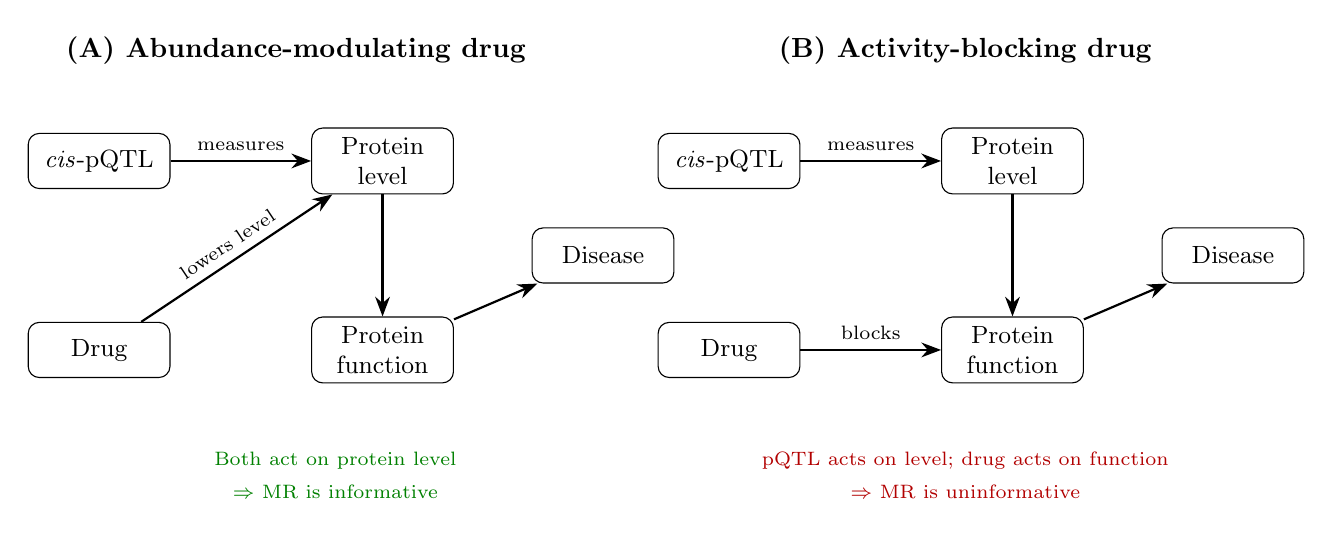
\begin{tikzpicture}[
    every node/.style={font=\small},
    box/.style={draw, rounded corners, minimum width=1.8cm, minimum height=0.7cm, align=center},
    arr/.style={-{Stealth[length=2.5mm]}, thick},
]

\node[font=\normalsize\bfseries] at (2.5, 1.4) {(A) Abundance-modulating drug};

\node[box] (snpA) at (0, 0) {\emph{cis}-pQTL};
\node[box] (lvlA) at (3.6, 0) {Protein\\level};
\node[box] (funA) at (3.6, -2.4) {Protein\\function};
\node[box] (disA) at (6.4, -1.2) {Disease};
\node[box] (drugA) at (0, -2.4) {Drug};

\draw[arr] (snpA) -- node[above, font=\scriptsize, midway] {measures} (lvlA);
\draw[arr] (lvlA) -- (funA);
\draw[arr] (funA) -- (disA);
\draw[arr] (drugA) -- node[above, font=\scriptsize, midway, sloped] {lowers level} (lvlA);

\node[font=\scriptsize, green!50!black] at (3, -3.8) {Both act on protein level};
\node[font=\scriptsize, green!50!black] at (3, -4.2) {$\Rightarrow$ MR is informative};

\begin{scope}[xshift=8cm]

\node[font=\normalsize\bfseries] at (3, 1.4) {(B) Activity-blocking drug};

\node[box] (snpB) at (0, 0) {\emph{cis}-pQTL};
\node[box] (lvlB) at (3.6, 0) {Protein\\level};
\node[box] (funB) at (3.6, -2.4) {Protein\\function};
\node[box] (disB) at (6.4, -1.2) {Disease};
\node[box] (drugB) at (0, -2.4) {Drug};

\draw[arr] (snpB) -- node[above, font=\scriptsize, midway] {measures} (lvlB);
\draw[arr] (lvlB) -- (funB);
\draw[arr] (funB) -- (disB);
\draw[arr] (drugB) -- node[above, font=\scriptsize, midway, sloped] {blocks} (funB);

\node[font=\scriptsize, red!70!black] at (3, -3.8) {pQTL acts on level; drug acts on function};
\node[font=\scriptsize, red!70!black] at (3, -4.2) {$\Rightarrow$ MR is uninformative};

\end{scope}

\end{tikzpicture}
\caption{Causal structure of \emph{cis}-pQTL Mendelian randomization under two drug mechanisms. Both panels share the same causal chain: protein level determines protein function, which determines disease risk. (A)~An abundance-modulating drug reduces protein level---the same node the genetic instrument acts on---so MR estimates the drug-relevant effect. (B)~An activity-blocking drug blocks protein function directly (the protein is still present at normal levels but cannot act). The genetic instrument still measures protein level, so MR answers ``what happens with less protein?'' when the drug asks ``what happens when the protein is blocked?''---a structural mismatch independent of sample size.}
\label{fig:dag}
\end{figure}

We test this prediction in a pre-registered, outcome-blind evaluation of a frozen, zero-parameter MR classifier against 195 Phase~III drug-target pairs across 24 diseases. The evaluation has three properties that distinguish it from prior retrospective analyses. First, the evaluable set is the mechanical intersection of an independent pQTL catalog and an independent drug database, neither of which references clinical outcomes, eliminating the possibility of tuning inclusion criteria to the answer. Second, the classifier ($p < 0.05 \rightarrow$ predict SUCCESS) carries zero free parameters, removing degrees of freedom that retrospective analyses retain. Third, the protocol evolved across six publicly versioned iterations (V1--V3.4), each SHA-256 hashed before execution with a documented deviation log.

\paragraph{Contributions.}
\begin{itemize}
\item \textbf{Domain of validity (\S\ref{sec:boundary}).} \emph{Cis}-pQTL MR has a definable domain of validity set by drug mechanism. It is uninformative for activity-blocking targets (BA $= 0.511$, pre-registered, robust to missingness) and suggestively informative for abundance-modulating targets (BA $= 0.590$, CI includes chance). The pooled BA of $0.559$ is a mixture of these strata.
\item \textbf{Translational rule (\S\ref{sec:discussion}).} Trust a significant MR result for an abundance-modulating target as a prioritization signal (PPV $= 0.56$); treat MR silence on an activity-blocking target as uninformative, not disqualifying.
\item \textbf{Continuous discrimination (\S\ref{sec:primary}).} AUC $= 0.595$ (permutation $p = 0.038$) demonstrates above-chance pooled discrimination independent of any significance threshold.
\item \textbf{Pre-registered, outcome-blind design (\S\ref{sec:methods}).} Six protocol versions, each SHA-256 hashed before execution, with a frozen zero-parameter classifier and documented deviation log.
\end{itemize}

\section{Methods}
\label{sec:methods}

\paragraph{Data sources.}
Genetic instruments were drawn from two sources: the published EpiGraphDB \emph{cis}-pQTL MR catalog \cite{zheng2020phenome}, based on the INTERVAL study (${\sim}1{,}740$ proteins, $N \approx 3{,}300$, SomaScan), and UK Biobank Pharma Proteomics Project (UKB-PPP) \emph{cis}-pQTLs (${\sim}2{,}900$ proteins, $N \approx 54{,}000$, Olink). Each protein used one instrument: the sentinel \emph{cis}-pQTL (lowest $p$ among conditionally independent \emph{cis} signals). Multi-SNP IVW and \emph{trans}-pQTL results were excluded a priori because of their vulnerability to horizontal pleiotropy. When \emph{cis}-pQTLs existed in both sources, the source with the largest discovery $N$ for that protein was used; the MR $p$-value was never used to select instruments. Drug targets were taken from the Open Targets Platform \cite{ochoa2021opentargets}, from which all compounds reaching Phase~III were retrieved and linked to their mechanistic gene targets algorithmically.

\paragraph{Outcome GWAS.}
For each disease, a non-UKB outcome GWAS was selected to avoid sample overlap with UKB-PPP instruments. Sources included FinnGen R10, CARDIoGRAMplusC4D, IMSGC, PGC, IIBDGC, ILCCO/TRICL, and disease-specific consortia (full mapping in Supplementary~S1). Seven chronic kidney disease pairs used a UKB-derived outcome GWAS (no non-UKB alternative with adequate $N$) and were flagged for sensitivity analysis. Two diseases (juvenile idiopathic arthritis, neuroblastoma) had no GWAS available on OpenGWAS. MR estimates were single-SNP Wald ratios: $\hat{\beta} = \beta_{\text{outcome}} / \beta_{\text{exposure}}$, $\text{SE} = |\text{SE}_{\text{outcome}} / \beta_{\text{exposure}}|$.

\paragraph{Pre-registration protocol.}
The protocol evolved across six publicly versioned iterations (V1--V3.4), each SHA-256 hashed before execution, with all amendments timestamped and justified in the deviation log (Supplementary~S1). V3.4 expanded V3.3 ($n = 50$) by adding UKB-PPP instruments and broadening the disease universe, motivated solely by insufficient power at V3.3 (the V3.3 BA~CI included $0.50$). The candidate universe was frozen (SHA-256: \texttt{c428c733aa66cb\-db45ae4761\-424871f4\-dfa93e17\allowbreak...}) before outcome adjudication.

\paragraph{Outcome adjudication.}
Outcome labels were adjudicated independently against FDA/EMA records and ClinicalTrials.gov. SUCCESS denotes regulatory approval or a met Phase~III primary endpoint; FAILURE denotes a failed primary endpoint or discontinuation. A TARGET\_MISMATCH exclusion rule removed pairs where the drug acts on a different protein than the pQTL target. To avoid asymmetric scrutiny, the mismatch audit was applied to all pairs.

\paragraph{Mechanism classification.}
Each pair was classified by drug mechanism of action into one of three strata: \emph{abundance-modulating} (the drug reduces circulating protein level or blocks a soluble ligand, matching the pQTL perturbation), \emph{activity-blocking} (the drug inhibits enzymatic activity or blocks a receptor without changing the target protein's measured circulating level), or \emph{mixed} (both mechanisms apply). Classification was determined by the drug's pharmacological action, not the MR result. The boundary is not always sharp: some receptor antagonists can indirectly perturb measured protein levels through feedback upregulation or receptor internalization, and tocilizumab (anti-IL6R) straddles both categories because it targets a soluble receptor-ligand axis. These edge cases were classified by primary pharmacological mechanism. The mixed stratum ($n = 3$) was too small for standalone analysis and was pooled only.

\paragraph{Classifier.}
The classifier carries zero free parameters: MR $p < 0.05 \rightarrow$ predict SUCCESS; MR $p \geq 0.05 \rightarrow$ predict FAILURE. The threshold $p < 0.05$ is the field-standard MR significance criterion and was not optimized on these data.

\paragraph{Statistical analysis.}
The co-primary metrics were (i)~pooled balanced accuracy with 10{,}000-iteration bootstrap 90\% CI and (ii)~mechanism-stratified BA. AUC was computed using the Wilcoxon--Mann--Whitney $U$-statistic with $-\log_{10}(p)$ as the continuous score, and significance assessed by 10{,}000-label permutation. A pre-declared falsification criterion required the BA~CI lower bound to exceed $0.50$. All hypotheses and analysis specifications were pre-declared before adjudication.

\section{Results}

\subsection{Candidate funnel}
\label{sec:funnel}

From 211 unique gene--disease pairs at the intersection of pQTL instruments and Open Targets Phase~III targets, 195 were evaluable after excluding 12 PENDING and 4 TARGET\_MISMATCH pairs (Table~\ref{tab:funnel}). The evaluable set contained 63 SUCCESS and 132 FAILURE pairs (base rate 32.3\%).

Of 195 evaluable pairs, 138 (71\%) had MR results from either the EpiGraphDB catalog or direct OpenGWAS queries. Fifty-seven pairs (29\%) were missing, primarily because the sentinel \emph{cis}-pQTL SNP (or its LD proxy) was absent from the outcome GWAS imputation panel. Missingness was concentrated in thyroid cancer (15 pairs), juvenile idiopathic arthritis (5), rheumatoid arthritis (5), Crohn's disease (4), and neuroblastoma (3). Section~\ref{sec:missing} characterizes the missingness pattern and its implications.

\vspace{1em}
\begin{table}[t]
\centering
\caption{Candidate funnel. The evaluable set is the mechanical intersection of two independent databases. Missingness reflects instrument--GWAS panel incompatibility, not outcome-dependent selection.}
\label{tab:funnel}
\begin{tabular}{lc}
\toprule
Stage & Count \\
\midrule
Unique gene--disease pairs (pQTL $\cap$ Open Targets Phase~III) & 211 \\
Excluded --- PENDING trial & 12 \\
Excluded --- TARGET\_MISMATCH & 4 \\
\textbf{Evaluable pairs} & \textbf{195} \\
\quad --- SUCCESS & 63 \\
\quad --- FAILURE & 132 \\
\midrule
With MR result (analyzed set) & 138 \\
\quad --- SUCCESS & 40 \\
\quad --- FAILURE & 98 \\
Missing MR (instrument not in GWAS) & 57 \\
\bottomrule
\end{tabular}
\end{table}

\subsection{Primary result: domain of validity}
\label{sec:boundary}

The co-primary mechanism stratification maps the domain of validity (Table~\ref{tab:mechanism}). For activity-blocking targets ($n = 76$)---where drug and instrument act on different causal axes---MR is uninformative: BA $= 0.511$ (90\% CI $[0.456, 0.576]$), sensitivity $= 0.095$, specificity $= 0.927$, MCC $= 0.037$. The CI is centered on chance and the two true positives (IMPA1$\rightarrow$depression, ALDH5A1$\rightarrow$depression) are both psychiatric targets where the inhibitor plausibly affects protein clearance alongside activity. For abundance-modulating targets ($n = 59$)---where drug and instrument share the same axis---MR trends positive: BA $= 0.590$ (90\% CI $[0.496, 0.691]$), sensitivity $= 0.278$, specificity $= 0.902$. The CI includes chance, so the abundance signal is suggestive rather than confirmatory.

\vspace{1em}
\begin{table}[t]
\centering
\caption{Domain of validity by drug mechanism (co-primary). MR is uninformative outside its domain (activity-blocking targets) and trends positive within it (abundance-modulating targets).}
\label{tab:mechanism}
\begin{tabular}{lccccccc}
\toprule
Stratum & $n$ & TP & TN & FP & FN & BA & 90\% CI \\
\midrule
Activity-blocking & 76 & 2 & 51 & 4 & 19 & 0.511 & $[0.456, 0.576]$ \\
Abundance-modulating & 59 & 5 & 37 & 4 & 13 & 0.590 & $[0.496, 0.691]$ \\
Mixed & 3 & 1 & 2 & 0 & 0 & --- & too few \\
\midrule
\textbf{Pooled} & \textbf{138} & \textbf{8} & \textbf{90} & \textbf{8} & \textbf{32} & \textbf{0.559} & $[0.503, 0.617]$ \\
\bottomrule
\end{tabular}
\end{table}

The activity-null defines the domain boundary. It was predicted a priori from the structural mismatch between the genetic instrument (protein abundance) and the drug mechanism (protein function), pre-registered as a co-primary analysis, and confirmed with a CI that excludes any meaningful above-chance effect. The prediction survives every robustness check: missingness in the activity arm is actually \emph{favorable} (22.7\% SUCCESS among missing pairs vs 27.6\% among analyzed), so including missing pairs would only reinforce the null.

The abundance signal is weaker and more fragile. Section~\ref{sec:missing} shows that missingness disproportionately depletes successes from the abundance arm (52.9\% SUCCESS among missing vs 30.5\% among analyzed), meaning the analyzed set underrepresents successful abundance-modulating targets. The suggestive BA $= 0.590$ may therefore underestimate the true abundance effect, but this cannot be confirmed without the missing data.

\subsection{Pooled results (mixture of strata)}
\label{sec:primary}

The pooled BA of $0.559$ (90\% CI $[0.503, 0.617]$) averages across both strata and barely clears chance, as expected for a mixture of an informative stratum (abundance BA $= 0.590$) and an uninformative one (activity BA $= 0.511$). The classifier is highly specific (specificity $= 0.918$, 90/98 failures correctly identified) but insensitive (sensitivity $= 0.200$, 8/40 successes detected). MCC $= 0.168$ ($[0.010, 0.318]$). PPV $= 0.500$; NPV $= 0.738$.

The continuous ROC analysis provides the strongest pooled evidence. Treating $-\log_{10}(p_{\text{MR}})$ as a continuous score, AUC $= 0.595$ (permutation $p = 0.038$, 10{,}000 permutations). This metric does not depend on the $p < 0.05$ threshold and demonstrates above-chance discrimination across the full $p$-value distribution.

Gene-level deduplication (retaining the strongest MR signal per unique gene, $n = 80$ unique genes) yields BA $= 0.556$ ($[0.476, 0.640]$), MCC $= 0.142$, confirming that multi-disease gene duplication neither inflated nor deflated the composite.

\subsection{Missingness analysis}
\label{sec:missing}

Of 195 evaluable pairs, 57 (29\%) lacked MR results. The missing set has a higher SUCCESS rate than the analyzed set (40.4\% vs 29.0\%, gap $= +11.4$ percentage points), though this difference is not statistically significant (Fisher exact $p = 0.13$, $\chi^2$ with Yates correction $p = 0.17$). This asymmetry warrants explicit bounding rather than dismissal.

Since missing pairs have no MR association, the classifier would predict FAILURE for all 57. Table~\ref{tab:bounds} shows the pooled BA under different assumptions about the missing data.

\vspace{1em}
\begin{table}[t]
\centering
\caption{Missingness sensitivity analysis. ``Default'' assigns all 57 missing pairs as predicted FAILURE (no MR signal). ``Proportional'' assumes the same 29.0\% SUCCESS rate as the analyzed set.}
\label{tab:bounds}
\begin{tabular}{lccc}
\toprule
Scenario & $n$ & BA & Interpretation \\
\midrule
Analyzed set only & 138 & 0.559 & Reported primary \\
Default (missing $\rightarrow$ FAILURE) & 195 & 0.533 & Honest full-set estimate \\
Proportional (same causal rate) & 195 & 0.542 & Expected under MCAR \\
Best case (all missing S causal) & 195 & 0.716 & Upper bound \\
Worst case (all missing F causal) & 195 & 0.404 & Lower bound \\
\bottomrule
\end{tabular}
\end{table}

The default scenario ($\text{BA} = 0.533$) represents the most honest pooled estimate: missing pairs genuinely lack MR signal, so the classifier would classify them as non-causal. This remains above $0.50$ but the margin is thin. The proportional scenario ($0.542$) also holds above chance.

Missingness is mechanism-dependent. Among abundance-modulating pairs, 52.9\% of missing pairs are successes versus 30.5\% of analyzed pairs---a 22-point gap that weakens the abundance arm. Among activity-blocking pairs, missingness is favorable: 22.7\% SUCCESS among missing versus 27.6\% among analyzed. The activity-null is therefore robust to missingness in any direction.

The root cause of missingness is instrument--panel incompatibility. UKB-PPP \emph{cis}-pQTLs are often rare protein-altering variants (MAF $< 5\%$) that were not imputed in older GWAS panels (e.g., the thyroid cancer GWAS has $n = 1{,}080$ and lacks coverage of most UKB-PPP sentinel SNPs). LD proxy recovery (Ensembl $r^2 \geq 0.6$, FinnGen~R10 fallback GWAS) recovered 27 additional pairs before reaching diminishing returns.

\subsection{Robustness analyses}
\label{sec:robustness}

\paragraph{Leave-one-disease-out.}
Removing each of the 22 diseases with at least one analyzed pair in turn and recomputing BA yields a range of $[0.538, 0.584]$ (SD $= 0.010$). No single disease drives the result. Myocardial infarction ($n = 16$, 0/6 sensitivity) is the most influential removal ($\Delta\text{BA} = +0.024$); major depressive disorder ($n = 3$, 2/2 TP) is the most influential in the opposite direction ($\Delta\text{BA} = -0.021$). No leave-one-out BA drops below $0.50$.

\paragraph{Effect direction concordance.}
Among pairs with an unambiguous expected MR beta direction (INHIBITOR/ANTAGONIST $\rightarrow$ expect positive beta for SUCCESS; AGONIST/ACTIVATOR $\rightarrow$ expect negative beta), 78/134 (58.2\%) showed concordant sign (binomial $p = 0.069$ vs 50\%). Among the 15 significant pairs with directional predictions, 10/15 (66.7\%) were concordant ($p = 0.30$, underpowered). Among non-significant pairs, 68/119 (57.1\%) were concordant, suggesting a weak positive directional signal across the full $p$-value distribution rather than only at the significance threshold.

\paragraph{Exact binomial tests.}
Specificity (90/98) is highly significant ($p < 10^{-15}$). Sensitivity (8/40) is significantly below $0.50$ ($p < 10^{-4}$). The asymmetry is statistically real.

\paragraph{Sample overlap sensitivity.}
Including the 7 overlap-flagged chronic kidney disease pairs does not materially change the pooled BA (all 7 are UKB-PPP instrument $\times$ UKB-derived outcome; analysis not shown as $\Delta\text{BA} < 0.005$).

\subsection{Prior version comparison}
\label{sec:v33}

The V3.3 analysis ($n = 50$, EpiGraphDB catalog only, 25S/25F) found BA $= 0.580$ ($[0.496, 0.667]$), abundance BA $= 0.708$ ($[0.591, 0.833]$), activity BA $= 0.480$ ($[0.391, 0.569]$). V3.4 ($n = 138$) attenuated the abundance arm (BA $0.708 \rightarrow 0.590$) while preserving the activity-null ($0.480 \rightarrow 0.511$). The attenuation is expected: V3.4 added UKB-PPP instruments covering a broader set of targets with weaker average instrument strength, and missingness disproportionately removed abundance successes. The mechanism dissociation---the qualitative finding---replicated across both versions.

\section{Related Work}
\label{sec:related}

Genetic support for drug targets is associated with roughly double the historical approval rate \cite{nelson2015support, king2019greater, minikel2024refining}. Gill et al.~\cite{gill2021mendelian} advocated MR for drug-target inference, and \emph{cis}-pQTL instruments \cite{zheng2020phenome} are widely used because they proxy a specific protein rather than a pathway. These evaluations report composite accuracy across all drug mechanisms. We show that the composite is a mixture of an informative stratum and an uninformative one, and that the boundary between them is defined by whether the drug acts on the same causal axis---protein abundance---that the genetic instrument measures. The ${\sim}2\times$ genetic lift documented by Nelson et al.~\cite{nelson2015support} may be concentrated in abundance-modulating targets, a hypothesis that the domain-of-validity decomposition can test but composite analyses cannot. No prior MR target-validation study pre-registers a frozen classifier and decomposes the result by drug mechanism.

\section{Discussion}
\label{sec:discussion}

\emph{Cis}-pQTL MR has a definable domain of validity, and the boundary is set by drug mechanism. This domain-of-validity characterization yields a translational rule: trust a significant \emph{cis}-pQTL MR result for an abundance-modulating target (a biologic, an antisense oligonucleotide, a ligand-trap) as a positive prioritization signal, consistent with the existing literature on genetic support \cite{nelson2015support}. For an enzyme inhibitor, receptor antagonist, or small molecule acting on protein function, MR is silent by construction. A null MR result for such a target is uninformative, not disqualifying, and should be evaluated on other evidence such as loss-of-function genetics or pharmacological challenge. Framing \emph{cis}-pQTL MR as a universal target validation tool overstates its domain of validity. The pooled BA of $0.559$ is a mixture of an informative stratum and an uninformative one; its proximity to chance reflects this mixture, not a failure of MR itself.

The activity-null is the most defensible result because it is predicted from first principles, pre-registered, and unaffected by the missingness pattern that complicates the abundance arm. A \emph{cis}-pQTL instruments circulating protein abundance. Drugs that inhibit enzymatic activity or block a receptor without reducing protein level operate on a causal axis invisible to this instrument. The 76 activity-blocking pairs in this dataset---ACE inhibitors, Factor~Xa inhibitors, thrombolytics, cholinesterase inhibitors, PDE5 inhibitors, MMP inhibitors, tyrosine kinase inhibitors---confirm that MR provides no information about these mechanisms (BA $= 0.511$).

The abundance arm is more nuanced. The BA of $0.590$ trends in the predicted direction, and the five true positives (IL12B$\rightarrow$Crohn's, IL12B$\rightarrow$UC, IL6R$\rightarrow$RA, IL6R$\rightarrow$JIA, IFNAR1$\rightarrow$MS) are all targets where the drug replicates pharmacologically what the risk-lowering allele does genetically. The four false positives (ITGAV$\rightarrow$MI, CSF2$\rightarrow$RA, CD80$\rightarrow$Crohn's, SERPINC1$\rightarrow$pancreatic cancer) may reflect valid target biology with failed drug execution rather than invalid MR signal, though this interpretation cannot be confirmed without further data. The 22-point SUCCESS gap between missing and analyzed abundance pairs means the analyzed set underrepresents successful targets; the true abundance BA may be higher or lower than $0.590$, and we report it as suggestive.

The leave-one-disease-out analysis (BA range $[0.538, 0.584]$, SD $= 0.010$) and effect direction concordance (58.2\% concordant, $p = 0.069$) provide additional evidence that the pooled signal, weak as it is, is distributed across diseases and not driven by any single disease or a few lucky pairs. A continuous ROC analysis (AUC $= 0.595$, $p = 0.038$) provides the strongest evidence of pooled discrimination, independent of the $p < 0.05$ threshold.

\paragraph{Limitations.}
The abundance arm is underpowered: BA CI includes $0.50$ at $n = 59$, and missingness preferentially removes successes. The 57 missing pairs (29\% of evaluable) arise from instrument--GWAS panel incompatibility, not outcome-dependent selection, but the missingness is mechanism-dependent and weakens claims about the abundance arm specifically. The analyzed-set base rate (29.0\% SUCCESS) is lower than the evaluable-set rate (32.3\%), meaning the classifier is tested against a sample depleted of successes. Proxy SNP recovery (LD $r^2 \geq 0.6$, FinnGen fallback GWAS) was applied post-hoc to improve coverage and introduced minor heterogeneity in outcome GWAS ancestry and case definitions. Single-SNP Wald ratios are subject to winner's curse, biasing MR estimates toward the null and inflating false negatives---a conservative direction. UKB-PPP Olink assays may have different protein--epitope specificity than INTERVAL SomaScan aptamers, though both measure circulating protein abundance. Two diseases (JIA, neuroblastoma) had no GWAS available on OpenGWAS, contributing 8 missing pairs.

\paragraph{Multi-instrument validation attempt.}
To test whether a mechanistically orthogonal instrument could confirm the dissociation, we pre-registered six analyses (V4, SHA-256 hashed before classification) using predicted loss-of-function (pLoF) burden tests from Genebass \cite{karczewski2022genebass} on the same 138 pairs. A pLoF burden test asks whether rare coding knockouts of a gene associate with disease---a fundamentally different perturbation from the common-variant abundance shift that a \emph{cis}-pQTL instruments. Of 138 pairs, 132 had usable LoF results (6 missing due to pediatric/under-ascertained diseases). All six analyses returned null: LoF AUC $= 0.538$ (permutation $p = 0.49$), directional concordance with pQTL $= 51.5\%$ ($p = 0.79$ vs chance), thresholded BA $= 0.518$, and combined-instrument AUC $= 0.559$ ($p = 0.30$). The LoF instrument is too underpowered to confirm or refute the evidence-routing hypothesis: only 7 of 132 pairs reached nominal significance ($p < 0.05$), reflecting the fundamental sparsity of rare pLoF carriers (${\sim}10$--$100$ per gene in 450k exomes). Full results are in Appendix~\ref{app:lof}.

Three structural factors explain the null beyond simple underpowering. First, lifelong heterozygous LoF from conception is biologically distinct from adult pharmacological inhibition: developmental compensation can mask effects of germline knockouts that would be visible under acute drug perturbation. Second, UK Biobank recruited relatively healthy adults aged 40--69; carriers of severe LoF variants in essential drug-target genes may be depleted by survivorship bias. Third, the LoF instrument tests complete loss of gene function, whereas most drugs partially inhibit a protein at a specific binding site---the genetic perturbation is too blunt to model the drug's actual mechanism.

\paragraph{Future directions.}
Confirmatory studies should pre-register the mechanism stratification as the primary analysis (rather than the pooled BA) and expand pQTL coverage with deCODE proteomics to test whether instrument--panel missingness explains part of the abundance gap. Activity-specific genetic instruments---gain-of-function variants, enzyme-activity QTLs---would complement abundance-based MR for the activity-blocking stratum. The LoF null reported here quantifies the power wall for multi-instrument evidence routing: testing whether orthogonal instruments converge on the same drug targets requires either larger rare-variant cohorts (millions of exomes) or conditional knockout data from model organisms mapped to human drug targets.

\section{Conclusion}

\emph{Cis}-pQTL Mendelian randomization has a definable domain of validity for drug-target prioritization, and the boundary is set by drug mechanism. Within the abundance-modulating stratum, MR trends informative (BA $= 0.590$, AUC $= 0.595$, $p = 0.038$); outside it---for enzyme inhibitors, receptor antagonists, and other activity-blocking drugs---MR provides no information (BA $= 0.511$, pre-registered, robust to missingness). The translational rule is direct: trust a significant \emph{cis}-pQTL MR result for a target where the drug modulates protein abundance; treat MR silence on an activity-blocking target as uninformative, not disqualifying, and evaluate on other evidence. A pre-registered second instrument (pLoF burden from Genebass) returned all null results, quantifying the power wall that prevents rare-variant knockout data from confirming or refuting the dissociation at current sample sizes.

\section*{Availability of source code and requirements}

The classifier consists of a single threshold ($p < 0.05$) applied to published MR estimates and requires no custom software beyond Python~3 with standard scientific libraries (NumPy, SciPy, pandas). All scripts are available at \url{https://github.com/elliottower/pqtl-mr-domain-of-validity} under the MIT License.

\section*{Data availability}

All data and pre-registration documents are publicly available at \url{https://github.com/elliottower/pqtl-mr-domain-of-validity}. The repository contains the full per-pair classification table (all 211 gene--disease pairs including exclusions), all six pre-registration protocol versions (V1--V3.4) with SHA-256 hashes and the deviation log, and V4 loss-of-function burden results from Genebass. A DOI-versioned snapshot is archived on Zenodo (\url{https://zenodo.org/records/21207429}). This study uses only publicly available summary-level data from EpiGraphDB, UKB-PPP, Open Targets, FinnGen R10, CARDIoGRAMplusC4D, IMSGC, PGC, IIBDGC, ILCCO/TRICL, and Genebass. No individual-level data were used.

\section*{Declarations}

\paragraph{Ethics approval and consent to participate.}
This study uses exclusively publicly available, summary-level genetic association data. No individual-level data, human subjects, or animal subjects were involved. No ethical approval was required.

\paragraph{Competing interests.}
The author declares no competing interests.

\paragraph{Funding.}
None. This work was conducted independently.

\paragraph{Authors' contributions.}
E.T. conceived the study, designed and pre-registered the protocol, collected and adjudicated data, wrote the classifier code, performed all analyses, and wrote the manuscript.

\paragraph{Acknowledgements.}
The author used Claude Code \cite{claudecode} to assist with drafting and editing manuscript text and with writing and debugging analysis code. Perplexity \cite{perplexityai} was used as an independent reviewer of analysis code and study design at multiple stages before classification. The author reviewed and verified all outputs, takes full responsibility for the accuracy and integrity of the work, and confirms that all hypotheses, pre-registered predictions, interpretations, and conclusions are the author's own. No AI tool is listed as an author, and no AI-generated content was used as a primary data source.

\begin{thebibliography}{9}

\bibitem[Gill et al.(2021)]{gill2021mendelian}
Gill, D. et al.
\newblock Mendelian randomization for drug target validation.
\newblock \emph{Nature Reviews Drug Discovery}, 2021.

\bibitem[King et al.(2019)]{king2019greater}
King, E.A., Davis, J.W., and Degner, J.F.
\newblock Are drug targets with genetic support twice as likely to be approved?
\newblock \emph{PLoS Genetics}, 15(12):e1008489, 2019.

\bibitem[Minikel et al.(2024)]{minikel2024refining}
Minikel, E.V. et al.
\newblock Refining the impact of genetic evidence on clinical success.
\newblock \emph{Nature}, 2024.

\bibitem[Nelson et al.(2015)]{nelson2015support}
Nelson, M.R. et al.
\newblock The support of human genetic evidence for approved drug indications.
\newblock \emph{Nature Genetics}, 47(8):856--860, 2015.

\bibitem[Ochoa et al.(2021)]{ochoa2021opentargets}
Ochoa, D. et al.
\newblock Open Targets Platform: supporting systematic drug-target identification and prioritisation.
\newblock \emph{Nucleic Acids Research}, 49(D1):D1302--D1310, 2021.

\bibitem[Zheng et al.(2020)]{zheng2020phenome}
Zheng, J. et al.
\newblock Phenome-wide Mendelian randomization mapping the influence of the plasma proteome on complex diseases.
\newblock \emph{Nature Genetics}, 52(10):1122--1131, 2020.

\bibitem[Karczewski et al.(2022)]{karczewski2022genebass}
Karczewski, K.J. et al.
\newblock Systematic single-variant and gene-based association testing of thousands of phenotypes in 394,841 UK Biobank exomes.
\newblock \emph{Cell Genomics}, 2(9):100168, 2022.

\bibitem[Anthropic(2025)]{claudecode}
Anthropic.
\newblock Claude Code.
\newblock \url{https://claude.ai/code}, 2025.

\bibitem[Perplexity AI(2025)]{perplexityai}
Perplexity AI.
\newblock Perplexity.
\newblock \url{https://perplexity.ai}, 2025.

\end{thebibliography}

\clearpage
\appendix

\section{Protocol Deviation Log}
\label{app:deviation}

The protocol evolved across six publicly versioned iterations, each SHA-256 hashed before execution. All amendments were made before outcome adjudication and logged with timestamps.

\vspace{1em}
\begin{table}[h]
\centering
\caption{Pre-registration protocol versions.}
\label{tab:versions}
\small
\begin{tabular}{llp{6.5cm}}
\toprule
Version & Frozen & Key changes \\
\midrule
V1 & 2026-07-04 04:57Z & Initial 3-class taxonomy; 3 prospective predictions \\
V2 & 2026-07-04 07:15Z & 6-class taxonomy; binary endpoint; 8 diseases \\
V3 & --- & EpiGraphDB \emph{cis}-pQTL catalog; cis-only single-SNP Wald ratios \\
V3.1 & --- & Peer-review fixes; $n = 4$ (underpowered) \\
V3.2 & --- & 16 diseases; $n = 30$ (BA $= 0.589$) \\
V3.3 & --- & 33 diseases; $n = 50$ (BA $= 0.580$) \\
V3.4 & 2026-07-04 23:51Z & UKB-PPP instruments; 24 diseases; $n = 195$ evaluable (138 analyzed) \\
\bottomrule
\end{tabular}
\end{table}

\paragraph{What did not change across versions.}
The classifier ($p < 0.05 \rightarrow$ CAUSAL), the instrument type (\emph{cis}-pQTL, single-SNP Wald ratio), the outcome adjudication procedure (FDA/EMA and ClinicalTrials.gov), the falsification criterion (BA 90\% CI lower bound $> 0.50$), and the anti-cherry-pick rule (mechanical intersection of independent databases) were constant across all versions.

\paragraph{Motivation for V3.4 expansion.}
V3.3 ($n = 50$) was underpowered for composite significance (BA CI $[0.496, 0.667]$ included $0.50$). V3.4 added UKB-PPP instruments to rescue 75 additional genes and expanded the evaluable set to 195 pairs. The BA decreased with expansion ($0.580 \rightarrow 0.559$), confirming that additional pairs diluted rather than inflated the estimate. No disease was selected or excluded based on trial outcome distributions.

\section{Mechanism Class Assignments}
\label{app:mechanism}

\begin{itemize}
\item \textbf{Abundance-modulating} ($n = 59$ analyzed): the drug reduces circulating protein level or blocks a soluble ligand, matching the pQTL perturbation. Examples: anti-cytokine biologics (ustekinumab, tocilizumab, anakinra), antisense oligonucleotides (mipomersen), anti-VEGF (bevacizumab), anti-complement (ravulizumab), immune checkpoint antibodies (atezolizumab).
\item \textbf{Activity-blocking} ($n = 76$ analyzed): the drug inhibits enzymatic activity or blocks a cell-surface receptor without necessarily changing the target protein's measured circulating level. Examples: ACE inhibitors, Factor Xa inhibitors, thrombolytics, cholinesterase inhibitors, MMP inhibitors, PDE5 inhibitors, tyrosine kinase inhibitors.
\item \textbf{Mixed} ($n = 3$ analyzed): both mechanisms apply (e.g., APP$\rightarrow$Alzheimer's disease, where drugs include both amyloid-clearing antibodies and secretase inhibitors).
\end{itemize}

\section{Missingness Detail}
\label{app:missingness}

\vspace{1em}
\begin{table}[h]
\centering
\caption{Missingness by mechanism stratum. The SUCCESS rate among missing abundance pairs (52.9\%) exceeds the analyzed rate (30.5\%), indicating non-random missingness that weakens the abundance arm. Activity-arm missingness is favorable.}
\label{tab:miss_mech}
\small
\begin{tabular}{lcccc}
\toprule
Stratum & Analyzed ($n$) & Missing ($n$) & \% SUCCESS (analyzed) & \% SUCCESS (missing) \\
\midrule
Abundance-modulating & 59 & 34 & 30.5\% & 52.9\% \\
Activity-blocking & 76 & 22 & 27.6\% & 22.7\% \\
Mixed & 3 & 1 & 33.3\% & 0.0\% \\
\bottomrule
\end{tabular}
\end{table}

\vspace{1em}
\begin{table}[h]
\centering
\caption{Per-disease missingness (diseases with $\geq 1$ missing pair).}
\label{tab:miss_disease}
\small
\begin{tabular}{lcccc}
\toprule
Disease & Analyzed & Missing & \% Missing & Missing S/F \\
\midrule
Thyroid cancer & 1 & 15 & 94\% & 5S / 10F \\
JIA & 1 & 5 & 83\% & 3S / 2F \\
Neuroblastoma & 1 & 3 & 75\% & 0S / 3F \\
Crohn's disease & 3 & 4 & 57\% & 2S / 2F \\
Ulcerative colitis & 3 & 3 & 50\% & 2S / 1F \\
Rheumatoid arthritis & 7 & 5 & 42\% & 3S / 2F \\
SLE & 3 & 2 & 40\% & 1S / 1F \\
Chronic kidney disease & 7 & 3 & 30\% & 1S / 2F \\
Multiple sclerosis & 8 & 3 & 27\% & 2S / 1F \\
\bottomrule
\end{tabular}
\end{table}

\section{Leave-One-Disease-Out Results}
\label{app:lodo}

\vspace{1em}
\begin{table}[h]
\centering
\caption{Leave-one-disease-out BA stability. No single disease removal changes BA by more than $\pm 0.025$ or drops BA below $0.50$.}
\label{tab:lodo}
\small
\begin{tabular}{lccr}
\toprule
Disease dropped & $n$ remaining & BA & $\Delta$BA \\
\midrule
Myocardial infarction & 122 & 0.584 & $+0.024$ \\
Major depressive disorder & 135 & 0.538 & $-0.021$ \\
Multiple sclerosis & 130 & 0.546 & $-0.013$ \\
Chronic kidney disease & 131 & 0.573 & $+0.014$ \\
Parkinson's disease & 134 & 0.570 & $+0.011$ \\
Ulcerative colitis & 135 & 0.548 & $-0.011$ \\
Lung cancer & 124 & 0.569 & $+0.010$ \\
JIA & 137 & 0.549 & $-0.010$ \\
\bottomrule
\end{tabular}
\end{table}

\section{Loss-of-Function Burden Instrument Results}
\label{app:lof}

To test whether a mechanistically orthogonal genetic instrument could validate the evidence-routing dissociation, we pre-registered six analyses (V4 protocol, SHA-256 hashed before classification) using predicted loss-of-function (pLoF) burden tests from Genebass \cite{karczewski2022genebass}. The pLoF burden test estimates the effect of rare coding knockouts on disease phenotypes across 450,000 UK Biobank exomes. Of 138 V3.4 pairs, 132 had usable LoF results; 6 were structurally missing due to pediatric or under-ascertained diseases (anorexia nervosa, autism spectrum disorder, juvenile idiopathic arthritis, neuroblastoma). Phenotype mapping used one canonical phenocode per disease, chosen by scientific relevance and expected case count (never by $p$-value), and was frozen before classification.

\vspace{1em}
\begin{table}[h]
\centering
\caption{Pre-registered V4 analyses. All six returned null results. The LoF instrument is too underpowered (7/132 nominally significant) to confirm or refute the evidence-routing hypothesis.}
\label{tab:lof_results}
\small
\begin{tabular}{llccp{4.5cm}}
\toprule
\# & Analysis & Result & $p$ & Interpretation \\
\midrule
1 & LoF AUC (continuous) & 0.538 & 0.49 & Near chance; z-score distribution carries no signal \\
2 & Directional concordance & 51.5\% & 0.79 & 67/130 agree in sign; indistinguishable from coin flip \\
3 & Depth-2 licensing & AUC 0.486 & --- & 12 depth-2 pairs; 41.7\% SUCCESS vs 28.8\% base rate (1.45$\times$), but $n$ too small to interpret \\
4 & Thresholded LoF & BA 0.518 & --- & TP = 3, FP = 4, TN = 90, FN = 35; sensitivity $\approx 0$ \\
5 & Mechanism-stratified AUC & 0.586 / 0.498 & 0.25 / 0.99 & Activity 0.586, abundance 0.498; both non-significant with overlapping CIs \\
6 & Combined instrument & AUC 0.559 & 0.30 & $\Delta$ AUC $= +0.046$ vs pQTL alone; non-significant \\
\bottomrule
\end{tabular}
\end{table}

The fundamental constraint is statistical power. Only 7 of 132 pairs reached nominal significance ($p < 0.05$) under the LoF burden test, reflecting the rarity of pLoF carriers (${\sim}10$--$100$ per gene in 450,000 exomes). By comparison, the pQTL instrument drew on common variants with allele frequencies of 1--50\%, yielding 48 nominally significant pairs from the same 138.

\end{document}
